\documentclass[a4paper, oneside]{discothesis}

\usepackage[utf8]{inputenc}
\usepackage[T1]{fontenc}

\usepackage{tikz}
\usepackage{pgfplots}

\usepackage{svg}

\usepackage{hyperref}
\usepackage{float}
\usetikzlibrary{pgfplots.groupplots}

%%%%%%%%%%%%%%%%%%%%%%%%%%%%%%%%%%%%%%%%%%%%%%%%%%%%%%%%%%%%%%%%%%%%%%%%%%%%%%%%%%%%%%%%%%%%%%%%%
% DOCUMENT METADATA

\thesistype{Semester Thesis} % Master's Thesis, Bachelor's Thesis, Semester Thesis, Group Project
\title{\textit{SwitP}: Mobile Application for Real-Time Swimming Analysis}


\author{Daniel Wirzberger Raimundo}
\email{wirdanie@student.ethz.ch}

\institute{Distributed Computing Group \\[2pt]
Computer Engineering and Networks Laboratory \\[2pt]
ETH Zürich}

% Optionally, you can put in your own logo here
%\logo{
\includegraphics[width=0.2\columnwidth]{figures/disco_logo_faded}}

\supervisors{Darya Melnyk, Simon Tanner\\[2pt] Prof.\ Dr.\ Roger Wattenhofer}

% Optionally, keywords and categories of the work can be shown (on the Abstract page)
%\keywords{Keywords go here.}
%\categories{ACM categories go here.}

\date{\today}

%%%%%%%%%%%%%%%%%%%%%%%%%%%%%%%%%%%%%%%%%%%%%%%%%%%%%%%%%%%%%%%%%%%%%%%%%%%%%%%%%%%%%%%%%%%%%%%%%

\begin{document}

\frontmatter % do not remove this line
\maketitle

\cleardoublepage

\begin{acknowledgements}
First of all, I want to thank Darya Melnyk and Simon Tanner for the insights they gave me during our weekly meetings and their feedback concerning this thesis.

I also want to thank the Aquatic Masters Team (AMT) Zürich for their flexibility, patience, and interest in this project. Special thanks go to their "coach" Beat Schilt, who was always ready to adapt the training to have more relevant data on the watch.

\end{acknowledgements}


\begin{abstract}
\textit{Smartwatches in the Pool} (SwitP) is an Android Wear application that implements the convolutional neural network (CNN) developed by Brunner et al.~\cite{BMSW19} to recognize swimming styles. Basing on the measurements from acceleration, rotation, and magnetic field sensors, this neural network can reliably predict what swimming style was swum.

The neural network itself is adapted to this mobile environment by using the Tensorflow Lite framework \cite{TFLite20}, which integrates both the conversion and prediction functions. Preprocessing functions, optimized for both embedded performance and adaptability to other functions, filter and resample the raw sensor data to make it usable by the CNN.

Using the resampled sensor data as well as the classification results, the application determines the number of lengths and the number of strokes that the swimmer has swum. A user interface gives live feedback and control to the swimmer and is designed to be used in the pool.
\end{abstract}

\tableofcontents

\mainmatter % do not remove this line

\chapter{Introduction}
Nowadays, smartwatches allow for the recognition of complex human activity, one of which being swimming in the pool. Traditionally (in commercially available sports watches), this is done using classical processing methods on the signals generated by the different sensors in the watches. This approach provides acceptable results but lacks some robustness and adaptability to the swimming abilities of the watch wearer. For example, if the swimmer has to slow down in a crowded lane, such methods might recognize one lap too much. Or if the swimmer has a weak wall push-off (often encountered in beginners), the watch might count one lap less. Furthermore, swimming style recognition is often limited, and the user often has to specify manually what style he is swimming.

The known flexibility of neural networks, and the possibility to improve their performance for a specific user, neural networks can provide a good solution to the swimming recognition problem. Recent progress in training methods and neural network integrability for low-power embedded devices, make them also a viable solution for real-time mobile applications.

Multiple works (some of them are introduced in Section~\ref{RelWork}) have investigated the recognition performance of such networks, but generally in an offline, high performance, artificial setup. 

In this specific project, the main goal is to be able to tell what the actual swimming style is in realtime on a smartwatch available on the public market, as well as count how many laps have been swum, while having a user-friendly interface. The neural network used for this project was designed and trained by Brunner et al.~\cite{BMSW19} (detailed in Section \ref{background}), and will be adapted to this embedded application.

The app designed during this thesis, and the project in general (which mainly consists of the app) will be referenced by SwitP, an abbreviation of \textit{Smartwatches in the Pool}.


\section{Related Work}\label{RelWork}
SwitP is mainly a continuation of the work presented in \cite{BMSW19}. This paper presents a method to acquire swimming data from a wrist-worn smartwatch, and structure it to train a specific neural network, which in turn can predict the swimming style with high precision. Furthermore, this work introduces a method to count laps based on the class predictions, which will also be used in SwitP. While this thesis aims to extend this project to provide real-time (on the smartwatch) classification and post-processing of the data, some modifications were brought to the original approach, they will be detailed in the upcoming chapters.

Wang~\cite{WANG19} also based on \cite{BMSW19} and aimed to extend the recognition capabilities beyond swimming styles and the pool, in the more general context of Human Activity Recognition (HAR). It also provided some insights as to what channels and sampling rates are relevant, as well as some alternative solutions for data-augmentation and stroke-counting methods. Furthermore, it has shown some limitations of the sensors available on the smartwatch.

Mooney et al.~\cite{MCGQ+15} provide an overview of different papers ($87$ in total) on swimming data acquisition and interpretation. This work shows some of the extensive research carried out in sensor selection and placement and compiles insights for the post-processing methods (lap detection and stroke counting will be discussed in Section \ref{PostProc}).

Siirtola et al.~\cite{SLR11} use discriminant analysis of the first and second-order to do an offline classification of swimming styles. They also show that depending on the sensor placement (on the upper back instead of the wrist), the estimation accuracy of specific swimming parameters can be increased. \cite{SLR11} also deals with lap and stroke counting, which will be discussed in \ref{PostProc}.

Pansiot et al.~\cite{PLY10} also use another sensor placement, on the swimmer's goggles. The analysis is done offline, after uploading the data stored in the accelerometer to another device. The swimming styles are recognized using k-Means clustering basing on the body angle values, computed from the acceleration values.

Further works and their solutions to specific problems will be introduced in the Sections which are most closely related to them.

\chapter{Background}\label{background}
The majority of the background is contained in \cite{BMSW19}, which is a paper detailing the data acquisition methods as well as the general Neural Network structure, training methods, and evaluation processes.

This chapter aims to summarize the main elements on which this project is based.
\section{General Network Structure}\label{genNetStruct}
The neural network structure used for this work is detailed in \cite[ch.4]{BMSW19}. Briefly, the input tensor is a $\mathtt{n\_ch}annels\times \mathtt{n\_sa}mples$ data frame, which is then passed through four convolutional layers accompanied by ELU activations and max-pooling, increasing the feature map depth to $64$, progressively reducing the height, but keeping a width of $\mathtt{n\_ch}annels$. Between these layers, $3\times 1$ convolution filters ensure data is not mixed between sensor channels. The last convolutional layer is connected to a $128$ units ELU-Activated fully connected layer, which is then connected to a softmax-activated $\mathtt{n\_cl}asses$ units fully connected layer, used as an output for class probabilities.


\begin{figure}[h]
    \centering
    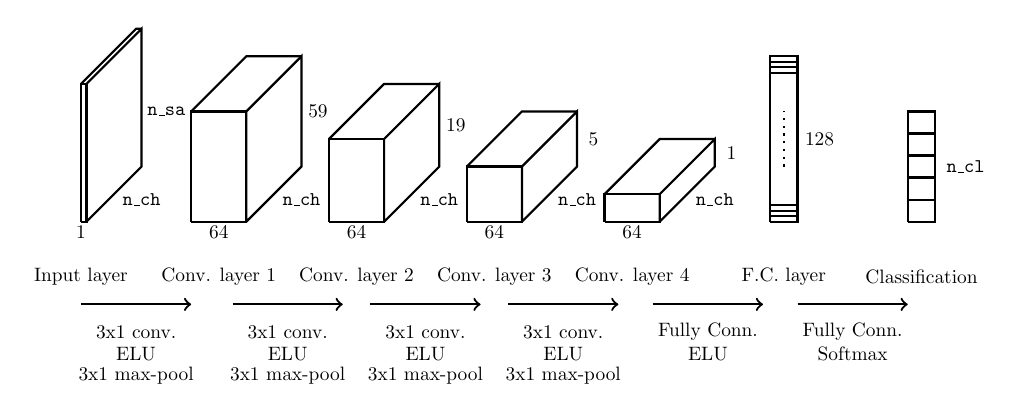
\begin{tikzpicture}[thick,scale=0.7, every node/.style={scale=0.7}]
\draw (0.5, 0) -- (0.6, 0) -- (0.6, 2.5) -- (0.5, 2.5) -- (0.5, 0);
\draw (0.6, 0) -- (1.6, 1.0) -- (1.6, 3.5) -- (0.6, 2.5) -- (0.6, 0);
\draw (0.5, 2.5) -- (1.5, 3.5) -- (1.6, 3.5);

\draw (2.5, 0) -- (3.5, 0) -- (3.5, 2) -- (2.5, 2) -- (2.5, 0);
\draw (3.5, 0) -- (4.5, 1.0) -- (4.5, 3.0) -- (3.5, 2) -- (3.5, 0);
\draw (2.5, 2) -- (3.5, 3.0) -- (4.5, 3.0);

\draw (5, 0) -- (6, 0) -- (6, 1.5) -- (5, 1.5) -- (5, 0);
\draw (6, 0) -- (7.0, 1.0) -- (7.0, 2.5) -- (6, 1.5) -- (6, 0);
\draw (5, 1.5) -- (6.0, 2.5) -- (7.0, 2.5);

\draw (7.5, 0) -- (8.5, 0) -- (8.5, 1) -- (7.5, 1) -- (7.5, 0);
\draw (8.5, 0) -- (9.5, 1.0) -- (9.5, 2.0) -- (8.5, 1) -- (8.5, 0);
\draw (7.5, 1) -- (8.5, 2.0) -- (9.5, 2.0);

\draw (10, 0) -- (11, 0) -- (11, 0.5) -- (10, 0.5) -- (10, 0);
\draw (11, 0) -- (12.0, 1.0) -- (12.0, 1.5) -- (11, 0.5) -- (11, 0);
\draw (10, 0.5) -- (11.0, 1.5) -- (12.0, 1.5);

\draw (13, 0) -- (13.5, 0) -- (13.5, 3) -- (13, 3) -- (13, 0);
\draw (13, 0.1) -- (13.5, 0.1);
\draw (13, 0.2) -- (13.5, 0.2);
\draw (13, 0.3) -- (13.5, 0.3);
\draw (13, 2.7) -- (13.5, 2.7);
\draw (13, 2.8) -- (13.5, 2.8);
\draw (13, 2.9) -- (13.5, 2.9);
\draw [dotted] (13.25, 1.0) -- (13.25, 2.0);

\draw (15.5, 0) -- (16, 0) -- (16, 2) -- (15.5, 2) -- (15.5, 0);
\draw (15.5, 0.4) -- (16, 0.4);
\draw (15.5, 0.8) -- (16, 0.8);
\draw (15.5, 1.2) -- (16, 1.2);
\draw (15.5, 1.6) -- (16, 1.6);

\draw (0.5,-0.2) node {1};
\draw (3,-0.2) node {64};
\draw (5.5,-0.2) node {64};
\draw (8,-0.2) node {64};
\draw (10.5,-0.2) node {64};

\draw (1.6, 0.4) node {\texttt{n\_ch}};
\draw (0.9+3.6, 0.4) node {\texttt{n\_ch}};
\draw (0.9+6.1, 0.4) node {\texttt{n\_ch}};
\draw (0.9+8.6, 0.4) node {\texttt{n\_ch}};
\draw (0.9+11.1, 0.4) node {\texttt{n\_ch}};

\draw (2.05, 2) node {\texttt{n\_sa}};
\draw (4.8, 2) node {59};
\draw (7.3, 1.75) node {19};
\draw (9.8, 1.5) node {5};
\draw (12.3, 1.25) node {1};
\draw (13.9, 1.5) node {128};
\draw (16.55, 1) node {\texttt{n\_cl}};

\draw (0.5,-1) node {Input layer};
\draw (3,-1) node {Conv. layer 1};
\draw (5.5,-1) node {Conv. layer 2};
\draw (8,-1) node {Conv. layer 3};
\draw (10.5,-1) node {Conv. layer 4};
\draw (13.25, -1) node {F.C. layer};
\draw (15.75, -1) node {Classification};

\draw (1.5, -2) node {3x1 conv.};
\draw (4.25, -2) node {3x1 conv.};
\draw (6.75, -2) node {3x1 conv.};
\draw (9.25, -2) node {3x1 conv.};
\draw (11.875, -2) node {Fully Conn.};
\draw (14.5, -2) node {Fully Conn.};
\draw (1.5, -2.4) node {ELU};
\draw (4.25, -2.4) node {ELU};
\draw (6.75, -2.4) node {ELU};
\draw (9.25, -2.4) node {ELU};
\draw (11.875, -2.4) node {ELU};
\draw (14.5, -2.4) node {Softmax};
\draw (1.5, -2.8) node {3x1 max-pool};
\draw (4.25, -2.8) node {3x1 max-pool};
\draw (6.75, -2.8) node {3x1 max-pool};
\draw (9.25, -2.8) node {3x1 max-pool};

\draw[->] (0.5, -1.5) -- (2.5, -1.5);
\draw[->] (3.25, -1.5) -- (5.25, -1.5);
\draw[->] (5.75, -1.5) -- (7.75, -1.5);
\draw[->] (8.25, -1.5) -- (10.25, -1.5);
\draw[->] (10.875, -1.5) -- (12.875, -1.5);
\draw[->] (13.5, -1.5) -- (15.5, -1.5);
\end{tikzpicture}
    \caption{Structure of the CNN used for recognition \cite{BMSW19}}
    \label{fig:ConvNet}
\end{figure}

The specific layer dimensions are primarily defined by the watch capabilities, but are also highly adaptable to the context:
\begin{itemize}
\item \texttt{n\_ch}, the number of sensor channels used as an input, is dependent on the sensors available on the watch, and on the number of channels each of them has (some of them returning a 3-axis triplet). As shown in \cite{WANG19}, networks based on fewer channels do not necessarily show worse precision. 
\item \texttt{n\_sa}, the number of samples used to build the input frame, can be determined by the sampling rate of the incoming signals (possibly resampled between sensors and neural network input), and the considered length of the input. In this project, the timing parameters were kept as in \cite{BMSW19}, namely $\mathtt{n\_sa}=180$ samples, and a sampling rate of $30~Hz$ for each channel, effectively making $6~s$ windows.
\item \texttt{n\_cl}, effectively the number of classes to be recognized at the output, is defined by the user, as the number of classes one wants to recognize. Here, we used $\mathtt{n\_cl}=5$, with the following classes (the enumeration numbers correspond to the output tensor ordering):
\begin{enumerate}
    \setcounter{enumi}{-1}
    \item \texttt{Null}: Default class, corresponding to resting periods and turns; 
    \item \texttt{Freestyle}: for classifying crawl;
    \item \texttt{Breaststroke};
    \item \texttt{Backstroke};
    \item \texttt{Butterfly}.
\end{enumerate}
\end{itemize}


\section{Training Method and Data}
\paragraph{Acquisition} The training data is acquired by equipping swimmers with the watch. During their training, the data provided by the different available sensors is stored on the watch, and generally, a person overseeing the training logs what specific swimming styles were swum (this can also be done by the swimmer himself, especially if he/she follows a specific program).

\paragraph{Labeling} In a second step, the data is first resampled and then manually labeled; each timestamp of the signal is assigned one of the previously mentioned classes. This is done by using a graphical tool (which has also been expanded during this project) to increase user-friendliness.

\paragraph{Training} To train the network, windows of sensor data of size $\mathtt{n\_ch}\times\mathtt{n\_sa}$ are prepared. At this step, the following methods are applied to increase the robustness of the algorithm, in this order:
\begin{itemize}
    \item \textit{time-scaling}: two copies $y_\alpha(t)$ of the original data $x(t)$ are generated, using $y_\alpha(t)=x(\alpha t)$, and with $\alpha \in \{0.9,1.1\}$;
    \item \textit{window-cutting}: at this step, the 3 (original and time-scaled) versions are separated into $\mathtt{n\_ch}\times\mathtt{n\_sa}$ windows. To always have a window having its center close to the classified timestamp, the windows overlap by $\frac{5}{6}\cdot \mathtt{n\_sa}$;
    \item \textit{normalization}: to avoid magnitude variations between swimmers, sensors and watches, each channel of each window is normalized;
    \item \textit{noise addition}: zero-mean Gaussian noise with a standard deviation of $1\%$ is added to each normalized window;
    \item \textit{measurement reversal}: to simulate the user wearing the watch on the other wrist, the additive inverse of channels $\mathtt{acc_x}, \mathtt{mag_x}, \mathtt{gyro_{y,z}}$ is used with a probability of $50\%$;
    \item \textit{measurement rotation}: for the tridimensional sensors, the windows are rotated by an angle $\theta$ uniformly sampled from the interval $[-\frac{\pi}{6},\frac{\pi}{6}]$, approximating the signals obtained by using a loosely worn watch.
\end{itemize}

Other techniques could be applied for further improvements, like time-reversal, some of them have been tested in \cite{WANG19}.

Finally, the neural network is trained by minimizing the negative log-likelihood on mini-batches consisting of 64 windows stratified across users and classes. All the available and valid (with one dominant class, and no unlabeled parts) windows are then used to train the network.

\chapter{SwitP Application}
The main result of this project is the application that will be presented in this chapter. It implements the original classification method, a graphical user interface as well as pre- and post-processing functions.

During development, priority was given to develop a user-friendly interface, keep the code simple and relatively efficient, as well as to make the implemented solutions compatible with other Android smartwatches. To avoid freezing the UI by overloading the main thread, and allow the scheduler to load balance across the multiple cores constituting the CPU (4 cores for the Snapdragon 2100 used in the Nixon the Mission), the computationally intensive tasks are run asynchronously in different threads.

The application was developed from scratch on a Nixon The Mission smartwatch \cite{Miss20}, which at the time runs Wear OS \texttt{2.17} and stock (non-unlocked nor rooted) Android \texttt{8.0.0}. The code is developed on Android Studio and stored/versioned/built (using continuous deployment) on:

\url{gitlab.ethz.ch/disco-students/fs20/smartwatches_swimming_daniel}

This repository also gives information on how to install the application on the watch. In the following, an overview of SwitP is given.

\section{General Structure}
The UI of the system, which also controls the whole backend, is mainly based on two screens (named activities in Android). 

Figure \ref{fig:flowchart} gives an overview of how these two activities are linked, as well as what parts are related to which activity. 
The first activity appears on the launch, just shows start/exit buttons, and a sliding drawer menu. This options menu allows to choose if data has to be "simulated" (use data from a specific file on the watch), what parameters have to be exported, as well as set up the length of the pool. 
The second one is related to the recording, and the only user input is whether the recording has to be stopped. This activity manages the backend lifecycle as and refreshes swimming parameters (number of strokes, of laps, total time) shown on the watch. 


The GUI is also discussed in Section \ref{test}.
\begin{figure}[H]
  \centering
  \includesvg[width=.89\linewidth]{figures/general_struct.svg}
  \caption{General SwitP flowchart}\label{fig:flowchart}
\end{figure}

The backend has been divided in multiple parts, which do the pre- and postprocessing of the data, and also handle the neural network. The chart shown in Figure \ref{fig:backendstruct} synthesizes the data flow going through the different steps, which are explained in the upcoming sections.
\begin{figure}[H]
  \centering
  \includesvg[width=.89\linewidth]{figures/back_struct.svg}
  \label{fig:backendstruct}
  \caption{Backend structure}
\end{figure}

\section{Preprocessing of the Sensor Data}\label{PreProc}
The preprocessing step mainly aims to format the input data to make it usable by the neural network. One main concern is that the sample rates can vary across devices and even sensors. Furthermore, the Android sensor stack \cite{SensStack20} does not allow precise setting of the sampling frequency (just a delay is given) and limits the performance of the embedded sensors \cite{SPAC+18}. To keep the program adaptable to other devices, this hardware abstraction layer was kept, and another abstraction layer, to preprocess the sensor data, is added.

For this project, the depth of the windows was defined (see Section \ref{genNetStruct}) as 180 normalized samples at $30~Hz$, which is what constrains the resampler output. In this specific case, the system was limited to three 3D sensors / 9 channels, namely accelerometer, gyroscope, and magnetometer, which are available on most commercial smartwatches (unlike light or pressure sensors), and have shown good precision in \cite{WANG19} and \cite{BMSW19}. Furthermore, keeping a small number of channels reduces power consumption, not only by actively polling fewer sensors but also by performing fewer tensor operations when using the neural network.

\paragraph{Resampling - original approach} Originally (in \cite{BMSW19}), the sampling rate problem is addressed by using cubic interpolation on the raw sensor signals, sampled at $100~Hz$ and $50~Hz$. While this solution is simple to implement for the training stage and still allows a good classification performance, it violates the Shannon-Nyquist sampling theorem (it can be related to downsampling, which introduces aliasing if not preceded by adapted filters).

\paragraph{Resampling - this thesis} First, the sampling rate is set as low as possible (while still $\geq 30~Hz$). The actual sampling rates on the Nixon the Mission are measured (by using the available timestamps) at $50~Hz$ for the magnetometer, and $~52~Hz$ for the accelerometer and gyroscope, which use the same measurements. These frequencies are then used to design a resampler, which first upsamples the signal, filters it (considering only the samples kept after decimation, for efficiency) to the output Nyquist frequency ($15~Hz$ in this case), and finally downsamples it. To be able to use the old (saved) as well as the new recordings, a few filters are designed for frequencies between $50~Hz$ and $104~Hz$, corresponding to the available sampling rates. These FIR equiripple filters are designed using the FilterDesigner tool in MATLAB, with a passband ripple of $0.4~dB$, a stopband attenuation of $20~dB$, and transition frequencies depending on the specific filter. For filters respecting these constraints with a small number of taps, the specificity of the constraints is artificially increased beyond the aforementioned characteristics to obtain a group delay of $195~ms\pm1~ms$ for all resamplers, ensuring the sensor signals are all in phase after filtering.

\paragraph{Window creation} A timer is used to create a new window every second, with the latest available data using the latest available timestamp across all sensor channels. This data is then normalized by channel, by computing the average and standard deviation of the $180$ selected samples. This step could be optimized, if the intermediate values needed for normalization were stored and updated, instead of computing them from scratch every time. However, as the measurement frequency can show small jitter, which in turn makes window length vary a bit, this would need a more complex approach to compensate for border effects.

\paragraph{Resampling for stroke counting} For stroke counting, the required sampling frequency is much lower, as the stroke rate of swimmers is limited (between $50-100$ strokes per minute depending on the style and distance), and therefore lower sampling rates retain most if not all of the necessary information. As the measurement is done on one arm only, a maximal frequency of about $0.8~Hz$ is expected, meaning the sampling frequency should be at least $1.6~Hz$. Nevertheless, Davey et al.~\cite{DAJ08} use a frequency of $0.5~Hz$ to do peak detection in realtime, while Chakravorti et al.~\cite{CSSC13} detect zero-crossings on a $1Hz$ sampling rate signal. The work of Bächlin and Tröster~\cite{BG11} is based on the gradient of a signal with a sampling rate of $2.56~Hz$. Finally, Wang~\cite{WANG19}, using the same watch as the one used for SwitP, shows that for cutoff frequencies between $1.5~Hz$ and $15~Hz$, also using different combinations of all the available sensors, the best results are obtained with the lowest frequencies. For this project, the sampling frequency of the signal used for stroke counting is set to $3~Hz$, and a filter with the same constraints as for the other resamplers is designed. To save on filter taps and computational load, the signal is resampled from the $30~Hz$ signal instead of the raw sensor output.

\section{Adaptation to a Mobile Application}
In \cite{BMSW19}, the neural network was designed to run on a fully-fledged Tensorflow install, which is not available on embedded devices. The TFLite framework \cite{TFLite20} allows converting a Tensorflow model into a TFLite model, which uses different data structures to store models, and is provided with interpreters to run it on mobile devices. This framework also allows different levels of optimization, ranging from the mentioned data structure optimization to detecting the range of activations and quantizing them to \texttt{uint8}, using appropriate scale factor and intercept. 

For this project, the classification speed of the watch was first evaluated using the TFLite Model Benchmark Tool \cite{TFLiteBench20} which generates an executable running the converted Neural Network with random inputs. While this is not a completely representative test, it allows estimating inference performance without having the preprocessing parts. For windows with $11$ channels and $180$ samples, the inference time was under $7~ms$ per evaluation (while theoretically, the maximum available time would be $1s$ to have every window ready exactly on time, without accounting for the rest of the application).

This successful test showed that the default settings of TFLite, with no quantization, on the specific Nixon the Mission smartwatch, run the inference fast enough to not require further optimizations.

\section{Postprocessing}\label{PostProc}

\paragraph{Lap counting}
A method for lap counting basing on the probability $p_0$ of the \texttt{Null} class is proposed in \cite[Ch. 4]{BMSW19}, and can be synthesized as follows:

First the clear (with marked transitions) laps are detected:
\begin{enumerate}
    \item Generate binary signal $r(t)$ by thresholding $p_0$ with threshold $\tau_p=0.5$ (active high);
    \item Filter out transitions for which the contiguous $r(t)<t_{min}^{(transition)}=6~s$;
    \item Filter out laps (for which $r(t)=0$) which are shorter than $t_{min}^{(lap)}=22~s$;
\end{enumerate}
This removes most of the false positives which can be detected when the swimmer is resting, or if the neural network predicts the \texttt{Null} class for a singular time point in the middle of a lap. However, it also removes turns which are too short, and also turns in which the network is less confident ($p_0$ small). This can lead to predictions of very long laps.

To avoid this, an upper bound of $t_{max}^{(lap)}=75~s$ is introduced, and if the time between two detected laps is higher than this bound, the lap is recovered by progressively reducing $t_{min}^{(transition)}$ and $\tau_p$, until the thresholding gives a new lap.

The original implementation of this method is designed to be run offline, meaning the initial three steps were applied to all timestamp-probability pairs first, and then missing transitions are detected for the whole signal. For this project, however, the goal is to have it running in real-time, so this setup was converted to a finite state machine, illustrated in Figure \ref{fig:lapfsm}

\begin{figure}[H]
  \centering
  \includesvg[width=.89\linewidth]{figures/lapfsm.svg}
  \caption{Finite State Machine for Lap Detection}
    \label{fig:lapfsm}
\end{figure}

If no laps have been detected for too long, a "missing lap detector" is started with the data that is missing turns (according to $t_{max}^{(lap)}=75~s$) as input, running asynchronously in the background.



\paragraph{Stroke counting} Basing on the $3~Hz$-resampled z-channel of the accelerometer, different approaches can be used to extract the number of strokes a swimmer does. 

The main goal is to have a computationally inexpensive approach which still shows robustness to changing swimming styles, intensities, and even watches.

Multiple authors use classical approaches for this task. Siirtola, et al.~\cite{SLR11} use measured data to determine a threshold level for detecting strokes, and remove spurious results by limiting the stroke rate to realistic values. Bächlin and Tröster~\cite{BG11} compute the gradient in a $0.2~s$ sliding window, and then use its maximums to determine both wall pushes and arm strokes. Chakravorti et al.~\cite{CSSC13} stream the data to a computer, which then filters the data and uses zero-crossing detection to find strokes. N.Davey, M.Anderson et al.~\cite{DAJ08} approach this task by first calculating the mean, finding minimas / maximas below / above the mean, and discarding false positives by removing peaks of same polarity not separated by a peak of opposite polarity.

Methods based on learning the data have also been developed, and use different approaches. Wang~\cite{WANG19} first filters the data, performs Principal Component Analysis to find the most useful channels, and then tunes a peak detector by using grid search against the manually counted strokes. Schmidt et al.~\cite{SASL19} use a convolutional neural network to detect peaks and the baseline in a more general signal processing context. They do so by using the available data to tune a "filter" constituted of a CNN, followed by a non-linear readout layer, and show its performance in synthetic contexts is better than optimized continuous wavelet filtering methods.

All the mentioned approaches make a compromise between hard-coding some thresholds, or needing specific data to optimize them during training. The method proposed in this project adds an adaptive component, also eliminating the need for a supplementary normalization layer. It is based on computing the $z$-Score, which is a statistical value indicating how far (in term of standard deviations $\sigma$) a specific sample $x$ is from a population with mean $\mu$. It is defined as:
\begin{equation*} z=\frac{x-\mu}{\sigma} \end{equation*}
Intuitively, having a large absolute value of the $z$-Score means the sample $x$ is an outlier, or part of a peak. To use this on real-time data, Van Brakel~\cite{JPVB16} proposed an adaptive method, which takes $3$ parameters:
\begin{itemize}
    \item $t_d$: dynamic threshold, number of standard deviations necessary to consider a sample as an outlier;
    \item $l$: lag, size of the window used for the computation of $\mu_i$ and $\sigma_i$;
    \item $q$: influence, between $0$ and $1$, a parameter for filtering the effect of new measurements.
\end{itemize}
A parameter $t_{s}$ was added for SwitP, which adds some noise tolerance by ensuring a minimum, non-adaptive, acceleration threshold has to be passed before a peak is signaled. $x_i$ is used to denote the $i^{th}$ input sample , while $y_i$ indicates if it is an outlier, and $p_i$ if it is considered as a peak (because groups of outliers can be contained in a single peak). Mathematically, the algorithm can be written as follows:

\begin{align*}
    \tilde{x_i} &= \begin{cases}
    x_i, i \in \{0,\dots, l-1\};\\
    q\cdot x_i + (1-q)\cdot x_i, otherwise.\\
    \end{cases}\\
    \mu_i &= \frac{\Sigma_{i-l+1}^{i}\tilde{x_{i}}}{l} \qquad \sigma_i = \sqrt{\frac{\Sigma_{i-l+1}^{i}\left(\tilde{x_{i}}^2 - \mu_i\right)^2}{l-1}}\\
    z_i &= \frac{\tilde{x_i}-\mu_i}{\sigma_i}\\
    y_i &= \begin{cases}
    1, z_i \geq max(t_d\cdot \sigma_i, t_s);\\
    0, otherwise.
    \end{cases}\qquad
    p_i = \begin{cases}
    1, y_i-y_{i-1}=1;\\
    0, otherwise.
    \end{cases}
\end{align*}

The small number of tests (discussed in Section \ref{test}) did not allow a precise setting of the $4$ parameters. Just as a baseline, values $t_d=2, t_s=0.25 , l=5 , q=0.15$ were chosen.

Figure \ref{fig:strokedetec} visually shows how these parameters affect the computation of the peaks, and the adaptive characteristics of the algorithm. It also shows how for slower rising peaks, the first of the outliers is selected, which is not necessarily the largest value.
\begin{figure}[H]
  \centering
  \includesvg[width=.95\linewidth]{figures/strokedetec.svg}
  \caption{Example of z-Score based stroke counting, with intermediate variables used for peak detection}
  \label{fig:strokedetec}
\end{figure}

\chapter{Testing}\label{test}
The testing of the different parts of SwitP could not be done as foreseen, as all pools closed before the app had been developed, and did not reopen for the testing to be performed as planned. Nevertheless, the basic functionality could be tested in multiple ways, which will be explained in this chapter.

A first testing method is to read existing recordings, unlabeled, and feed them through the data pipeline shown in Figure \ref{fig:backendstruct} (replacing the "Measurement" block). This is done by using the "simulate" option in the menu shown in Figure \ref{fig:screens} (b).
Specific data fields (selected using the same options menu) can then be exported to a \texttt{.csv} file, making the data available for further analysis. As an example, Figure \ref{fig:test} is based on a recording done in 2018, during which the $4$ recognized swimming styles were swum over $50~m$ each, two times in a row.

\begin{figure}[H]
  \centering
  \includesvg[width=.95\linewidth]{figures/example.svg}
  \caption{Returned values on a $2\cdot 200~m$ medley}
  \label{fig:test}
\end{figure}

Figure \ref{fig:test} shows that the raw predicted classes are generally very close to the manual labels for this user (which was excluded from the training set). The predictions could be improved by implementing some smoothing, looking at estimations from window covering the same timespan, or by classifying more than once a second, and also using some kind of averaging. The lower part of Figure \ref{fig:test} shows that for this training set, the laps were recognized correctly. The stroke recognition part shows inconsistent results, but as discussed before, it needs some fine-tuning to provide good results. 

While the user interface could not get thoroughly tested and reviewed by persons external to the project, it proved to be well usable in the pool. Figure \ref{fig:screens} shows some of the most important menus appearing on the watch. The start and stop buttons have to be pressed and held during a certain time, during which a loading circle is displayed (as seen in (c)), after which a confirmation screen like in (d) is shown, to ensure no false deactivations are made in the pool.
\begin{figure} [H]
\centering
\begin{tabular}{cccc}
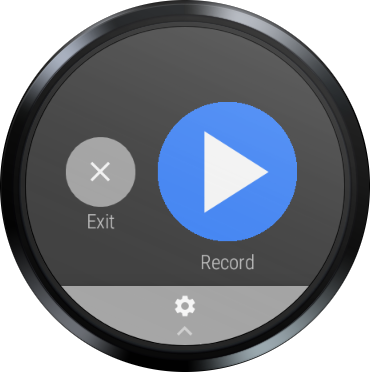
\includegraphics[scale=1.1]{figures/app/startmenu.png} &
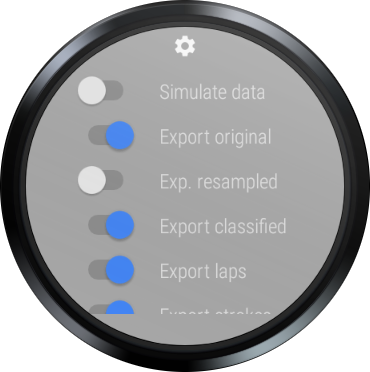
\includegraphics[scale=1.1]{figures/app/optionsmenu.png} \\
\textbf{(a)}  & \textbf{(b)} \\[6pt]
\end{tabular}
\begin{tabular}{cccc}
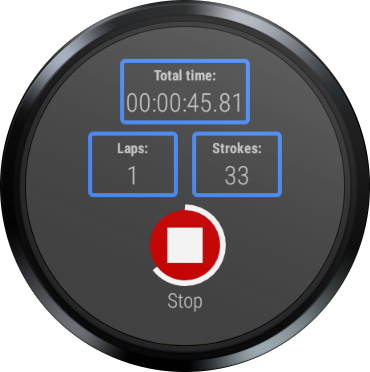
\includegraphics[scale=1.1]{figures/app/record.png} &
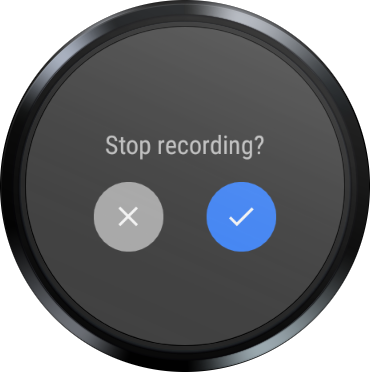
\includegraphics[scale=1.1]{figures/app/exitmenu.png} \\
\textbf{(c)}  & \textbf{(d)}  \\[6pt]
\end{tabular}
\caption{Screenshots of the SwitP application:
\textbf{(a)} Start menu
\textbf{(b)} Options drawer
\textbf{(c)} Recording screen
\textbf{(d)} Confirmation screen}
\label{fig:screens}
\end{figure}
Per default, Android applications all support backswipe to change activities, but also to exit an application. As this function can also be wrongly activated by pool water passing on the screen, for SwitP backswipe is disabled, and the exit button (as shown in (a)) is used to exit the application. The only physical button available on the Nixon the Mission used for this project still has its default function, namely returning to the main menu.

Finally, the last tests show that while putting the watch in airplane and battery saver modes increases its autonomy by several days, it also temporarily hangs the app and measurements, which should be addressed in the next iteration of SwitP development.

\chapter{Conclusions}
SwitP implements the convolutional neural network developed by Brunner et al.~\cite{BMSW19} to recognize swimming styles on an Android smartwatch. Using only the rotation, acceleration, and magnetic field sensors (available on most modern devices), this neural network can reliably predict what swimming style was swum.

The conversion of the neural network for mobile applications is done by using the Tensorflow Lite framework \cite{TFLite20}, which integrates both the conversion and prediction functions. Beforehand, the raw data produced by the sensors is filtered and resampled to be usable by the neural network, which is done by using an implementation optimized both for embedded performance and for adaptability to other watches.

The classification results as well as the resampled data are then used to determine the number of lengths and the number of strokes that the swimmer has swum. Finally, a user interface is added to the application, designed to be used in the pool and giving live feedback to the swimmer.

\section{Future Work}
A structured user-test of SwitP would help improving the application. On one hand, letting the interface be used by persons external to the project will test its ergonomy. On the other hand, these tests are required to fine-tune the adaptable parameters (e.g for stroke-counting) and get reliable results.

The adaptability of the preprocessing system can be increased, by automatically choosing the optimal sampling rates and resampler settings. This will remove the necessity to change these parameters between watches. As mentioned in Section \ref{PreProc}, the window creation method can be made more efficient by implementing a "rolling" system, instead of computing everything from scratch every time.

The convolutional neural network itself can be improved in multiple ways. First, using more training data, the kicking exercises done by swimmers might be recognizable as a new class. Secondly, more data augmentation techniques, such as those tested by Wang~\cite{WANG19}, could increase its precision.

Finally, the training experience could be improved by allowing programming of stuctured workouts, with a live training progress indicator in the watch UI.


% This displays the bibliography for all cited external documents. All references have to be defined in the file references.bib and can then be cited from within this document.
\bibliographystyle{IEEEtran}
\bibliography{references}

% This creates an appendix chapter, comment if not needed.
\appendix
%\chapter{First Appendix Chapter Title}

\end{document}